\documentclass[french]{article}
\usepackage[T1]{fontenc}
\usepackage[utf8]{inputenc}
\usepackage{lipsum}
\usepackage{lmodern}
\usepackage{geometry}
\usepackage{babel}
\usepackage{graphicx}
\usepackage{lastpage}
\usepackage{ragged2e}
\usepackage{enumitem}
\usepackage[normalem]{ulem}
\usepackage{hyperref} % pour \url{URL}
\usepackage{color} % pour \textcolor{color}{text}
\usepackage{listings} % pour afficher du code
\usepackage{longtable} % pour l'environnement longtable
\usepackage{float} % pour des figures non flottantes
\usepackage{amsmath}
\usepackage{verbatim} % pour les graphes
\usepackage{caption} % figure et subfigure pour mettre les images côtes à côtes
\usepackage{subcaption}
\usepackage{dirtree}
\usepackage{pdfpages}
% Pdf
\setboolean{@twoside}{false}

% Grammaire EBNF
\usepackage{syntax}
\setlength{\grammarparsep}{5pt plus 1pt minus 1pt}
\setlength{\grammarindent}{11em}

% Dessin avec tikz
\usepackage{tikz}
\usetikzlibrary{shapes,arrows,positioning,shadows,matrix,automata}

% Matrices
\usepackage{kbordermatrix}% http://www.hss.caltech.edu/~kcb/TeX/kbordermatrix.sty

% Largeur de colonnes de tableau fixes
\usepackage{array}
\newcolumntype{L}[1]{>{\raggedright\let\newline\\\arraybackslash\hspace{0pt}}m{#1}}
\newcolumntype{C}[1]{>{\centering\let\newline\\\arraybackslash\hspace{0pt}}m{#1}}
\newcolumntype{R}[1]{>{\raggedleft\let\newline\\\arraybackslash\hspace{0pt}}m{#1}}


% CSS
\lstdefinelanguage{CSS}{
	keywords={color,background-image:,margin,padding,font,weight,display,position,top,left,right,bottom,list,style,border,size,white,space,min,width, transition:, transform:, transition-property, transition-duration, transition-timing-function},	
	sensitive=true,
	morecomment=[l]{//},
	morecomment=[s]{/*}{*/},
	morestring=[b]',
	morestring=[b]",
	alsoletter={:},
	alsodigit={-}
}

% JavaScript
\lstdefinelanguage{JavaScript}{
	morekeywords={typeof, new, true, false, catch, function, return, null, catch, switch, var, if, in, while, do, else, case, break, let},
	morecomment=[s]{/*}{*/},
	morecomment=[l]//,
	morestring=[b]",
	morestring=[b]',
	morestring=[s]{/[}{/;}
}

\lstdefinelanguage{HTML5}{
	language=html,
	sensitive=true,	
	alsoletter={<>=-},	
	morecomment=[s]{<!-}{-->},
	tag=[s],
	otherkeywords={
		% General
		>,
		% Standard tags
		<!DOCTYPE,
		</html, <html, <head, <title, </title, <style, </style, <link, </head, <meta, />,
		% body
		</body, <body,
		% Divs
		</div, <div, </div>, 
		% Paragraphs
		</p, <p, </p>,
		% scripts
		</script, <script,
		% More tags...
		<canvas, /canvas>, <svg, <rect, <animateTransform, </rect>, </svg>, <video, <source, <iframe, </iframe>, </video>, <image, </image>, <header, </header, <article, </article
	},
	ndkeywords={
		% General
		=,
		% HTML attributes
		charset=, src=, id=, width=, height=, style=, type=, rel=, href=,
		% SVG attributes
		fill=, attributeName=, begin=, dur=, from=, to=, poster=, controls=, x=, y=, repeatCount=, xlink:href=,
		% properties
		margin:, padding:, background-image:, border:, top:, left:, position:, width:, height:, margin-top:, margin-bottom:, font-size:, line-height:,
		% CSS3 properties
		transform:, -moz-transform:, -webkit-transform:,
		animation:, -webkit-animation:,
		transition:,  transition-duration:, transition-property:, transition-timing-function:,
	}
}

\lstdefinestyle{htmlcssjs} {%
	% General design
	%  backgroundcolor=\color{editorGray},
	basicstyle={\footnotesize\ttfamily},   
	frame=b,
	% line-numbers
	xleftmargin={0.75cm},
	numbers=left,
	stepnumber=1,
	firstnumber=1,
	numberfirstline=true,	
	% Code design
	identifierstyle=\color{black},
	keywordstyle=\color{blue}\bfseries,
	ndkeywordstyle=\color{black}\bfseries,
	stringstyle=\color{red}\ttfamily,
	commentstyle=\color{gray}\ttfamily,
	% Code
	language=HTML5,
	alsolanguage=JavaScript,
	alsodigit={.:;},	
	tabsize=2,
	showtabs=false,
	showspaces=false,
	showstringspaces=false,
	extendedchars=true,
	breaklines=true,
	% German umlauts
	literate=%
	{Ö}{{\"O}}1
	{Ä}{{\"A}}1
	{Ü}{{\"U}}1
	{ß}{{\ss}}1
	{ü}{{\"u}}1
	{ä}{{\"a}}1
	{ö}{{\"o}}1
}
%
\lstdefinestyle{py} {%
	language=python,
	literate=%
	*{0}{{{\color{lightred}0}}}1
	{1}{{{\color{lightred}1}}}1
	{2}{{{\color{lightred}2}}}1
	{3}{{{\color{lightred}3}}}1
	{4}{{{\color{lightred}4}}}1
	{5}{{{\color{lightred}5}}}1
	{6}{{{\color{lightred}6}}}1
	{7}{{{\color{lightred}7}}}1
	{8}{{{\color{lightred}8}}}1
	{9}{{{\color{lightred}9}}}1,
	basicstyle=\footnotesize\ttfamily, % Standardschrift
	numbers=left,               % Ort der Zeilennummern
	%numberstyle=\tiny,          % Stil der Zeilennummern
	%stepnumber=2,               % Abstand zwischen den Zeilennummern
	numbersep=5pt,              % Abstand der Nummern zum Text
	tabsize=4,                  % Groesse von Tabs
	extendedchars=true,         %
	breaklines=true,            % Zeilen werden Umgebrochen
	keywordstyle=\color{blue}\bfseries,
	frame=b,
	commentstyle=\color{brown}\itshape,
	stringstyle=\color{editorOcher}\ttfamily, % Farbe der String
	showspaces=false,           % Leerzeichen anzeigen ?
	showtabs=false,             % Tabs anzeigen ?
	xleftmargin=17pt,
	framexleftmargin=17pt,
	framexrightmargin=5pt,
	framexbottommargin=4pt,
	%backgroundcolor=\color{lightgray},
	showstringspaces=false,      % Leerzeichen in Strings anzeigen ?
}%

\geometry{
	a4paper,
	total={210mm,297mm},
	left=20mm,
	right=20mm,
	top=20mm,
	bottom=20mm,
}

\usepackage{fancyhdr}
\pagestyle{fancy}
\setlist[enumerate,1]{leftmargin=2cm}

% Entêtes
\lhead{Champion, Loiseau\\Rochat, Schubert}
\chead{}
\rhead{PDG: Rapport}
\renewcommand{\headrulewidth}{0.4pt}
\renewcommand{\footrulewidth}{0.4pt}

\begin{document}
	
	
	% Titre du document
	\title{Projet Rady} % ou un autre nom\centering
	\author{Rapport\\ 
		Projet de groupe\\
		Champion, Loiseau, Rochat, Schubert\\
		Resp. René Rentsch\\
		HEIG-VD}
	\date{\today} % date du jour
	\maketitle
	\vspace{2cm}
	\centering
	
\includegraphics[scale=0.3]{../logo/icone}
	\thispagestyle{empty}
	
	\newpage
	\thispagestyle{empty}
	$ $
	\newpage
	
	% Pour tout le document
	\justify
	\normalsize
	
	% Tables des matières
	\tableofcontents
	
	\newpage
	
	\section*{Remerciements}
	Nous tenons tout d'abord à remercier M. Prof. René Rentsch pour son suivi et ses conseils durant toute la période du travail. Nous voulons également M. Prof. Olivier Liechti pour son aide dans le choix des technologies.
	
	\section{Introduction}
	Dans le cadre du cours PDG en troisième année du cursus de Bachelor de la HEIG-VD, il a été demandé de réaliser un projet de semestre sur une période de 10 semaines. Après l'acceptation du cahier des charges à la semaine 4, le projet a pu débuter. Celui-ci porte sur la réalisation d'une application mobile permettant permettant de se retrouver facilement entre amis notamment lors d'évènements. L’application se présenterait sous la forme d’une liste d’amis, laquelle permettrait de créer des groupes et de lancer une géolocalisation. L’utilisateur aurait alors le choix entre une carte en vue du dessus ou une boussole indiquant la direction à
	prendre.
	
		\subsection{Objectif}
		Les objectifs principaux de notre application peuvent être décomposés en trois grandes parties. Premièrement, la gestion des utilisateur, qui comprends la création de compte, la gestion de ce dit compte, ainsi que la recherche et l'ajout d'amis. Ensuite, l'intégration de la géolocalisation dans notre application doit permettre, par des appels API, aux utilisateurs de se retrouver. Cela constitue la partie centrale de l'application. Enfin étant donné des informations sensibles transiteront sur le réseau par le biais de notre application.\\
		Toutes les spécifications précises sont disponibles dans le cahier des charges fourni en annexe.
		
		\subsection{Architecture}
		L’application est composée d’une partie cliente (l'application mobile a proprement parlé), d’un serveur (hébergé sur une machine distante) communiquant avec une base de donnée et faisant appel au service FireBase Cloud Messaging (voir \textbf{figure \ref{Architecture simplifié}}). Le serveur sera à même de gérer la connexion et l’interaction avec plusieurs clients simultanément de manière transparente pour les utilisateurs. 
		Les données de l’application seront stockées dans une base de données dont l’accès direct se fera uniquement par le serveur. Les clients devront passer par l'API mise à disposition par le serveur pour tout accès aux données, pour des raisons évidentes de sécurité.
		Enfin le serveur fera appel au service FireBase Cloud Messaging (FCM) pour envoyer les notifications de push aux utilisateurs de l'application. 
		
		\begin{figure}[H]
			\centering
			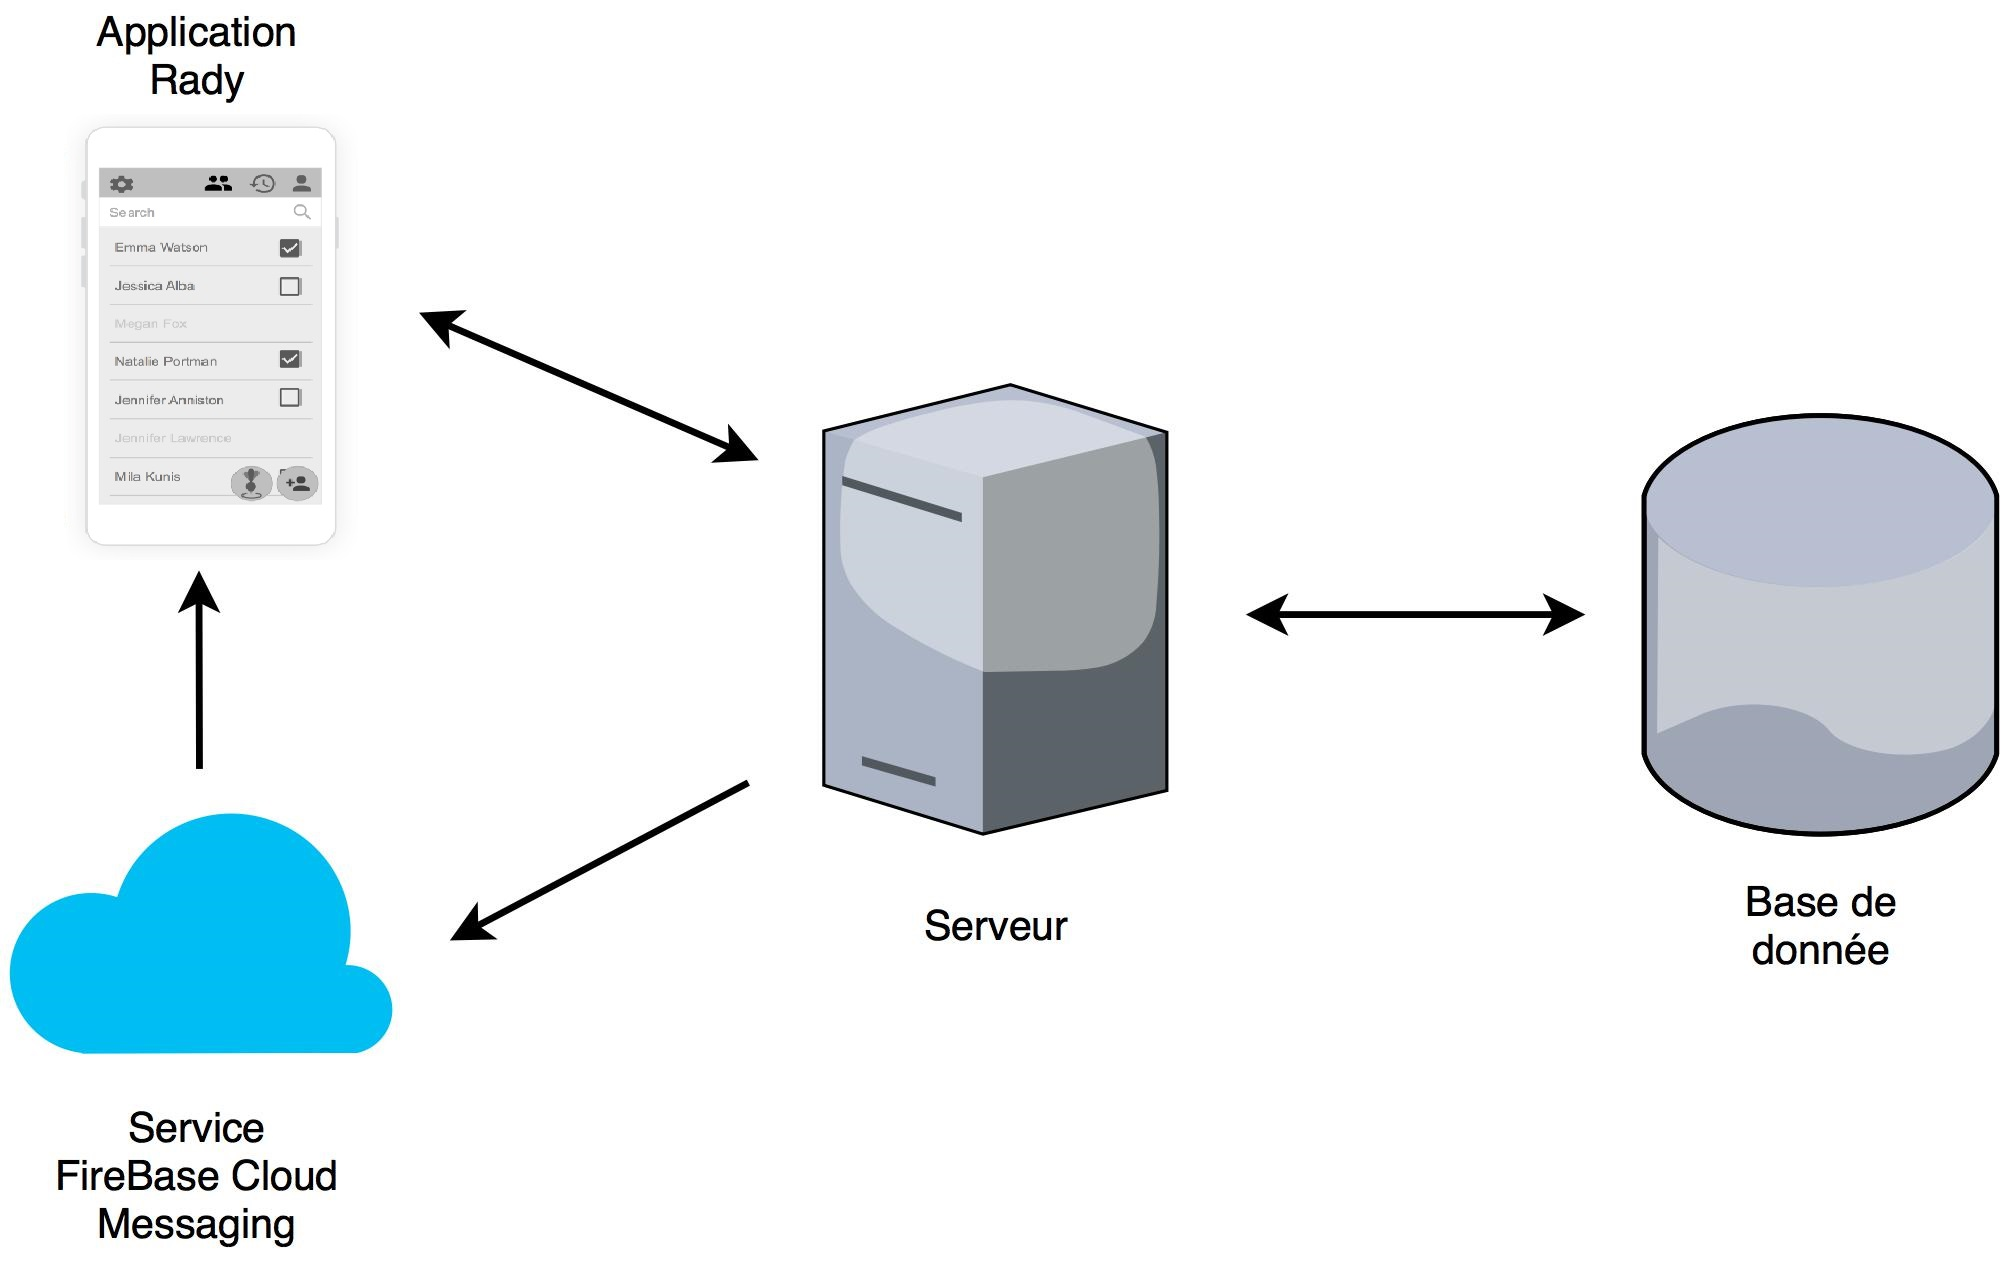
\includegraphics[scale=0.20]{../schema/schema-simplifie.jpg}
			\caption{Architecture simplifié}
			\label{Architecture simplifié}
		\end{figure}
		
		La conception générale de l'application a été divisé dans ces mêmes différentes parties afin de réduire les dépendances au niveau du développement (temps d'attente sur le travail des autres) ainsi que le nombre de conflit sur le gestionnaire de version.
		
		\subsection{Choix des technologies}
		Le choix des technologie a été un point clé lors de l'élaboration du cahier des charges et les premières étapes du développement à proprement parlé du projet.
		Nous avons essayer de choisir les technologies de manières à ce qu'elles soient maintenable, performantes.
		\begin{itemize}
			\item \textbf{Interface :} Pour l'interface nous pensions tout d'abord à utiliser \textbf{MeteorJS} \cite{meteor}, étant donné qu'il s'agit d'un framework pemettant un developpement "cross-plateform" performant. Cependant notre choix s'est finalement porté sur un autre framework "cross-plateform" \textbf{Ionic2} \cite{ionic} étant donné que \textbf{MeteorJS} est un framework dit "fullstack". Cela signifie qu'on aurait du développer avec ce framework de bout en bout, ce qui aurait pu compromettre le développement en cas de difficulté sur une des parties.
			\item \textbf{Serveur :} Concernant le serveur nous avons choisit d'utiliser \textbf{Django} \cite{django}  pour ses performances, sa sécurité, sa scalabilité et sa maintenabilité.
			\item \textbf{Base de donnée :} Le choix de la base de donnée s'est porté sur \textbf{PostgreSQL} car ce système de gestion de base de données (SGBD) est stable, fonctionne sur de nombreux OS et peut stocker des types de données dit "modernes". De plus ce SGDB fait parti des plus conforme aux norme ANSI SQL.
			\item \textbf{Serialisation :} Pour la sérialisation des données et leur transfert nous avons opté pour \textbf{JSON} car en comparaison avec \textbf{XML}, le \textbf{JSON} est plus léger, plus simple et peut directement être utilisé par le TypeScript et stocké tel quel dans le SGBD.
			\item \textbf{Notifications :} Le systeme de notification permettant au serveur de maintenir les utilisateurs à jour concernant les interactions inter-utilisateur se fera via \textbf{Firebase Cloud Messsaging}. FCM  repose sur le Google Cloud Messaging et nous offre un service de transmission de message fiable, une plus grande simplicité de developpement ainsi qu'une prise en charge multi-plateforme 
		\end{itemize}
		
		\begin{figure}[H]
			\centering
			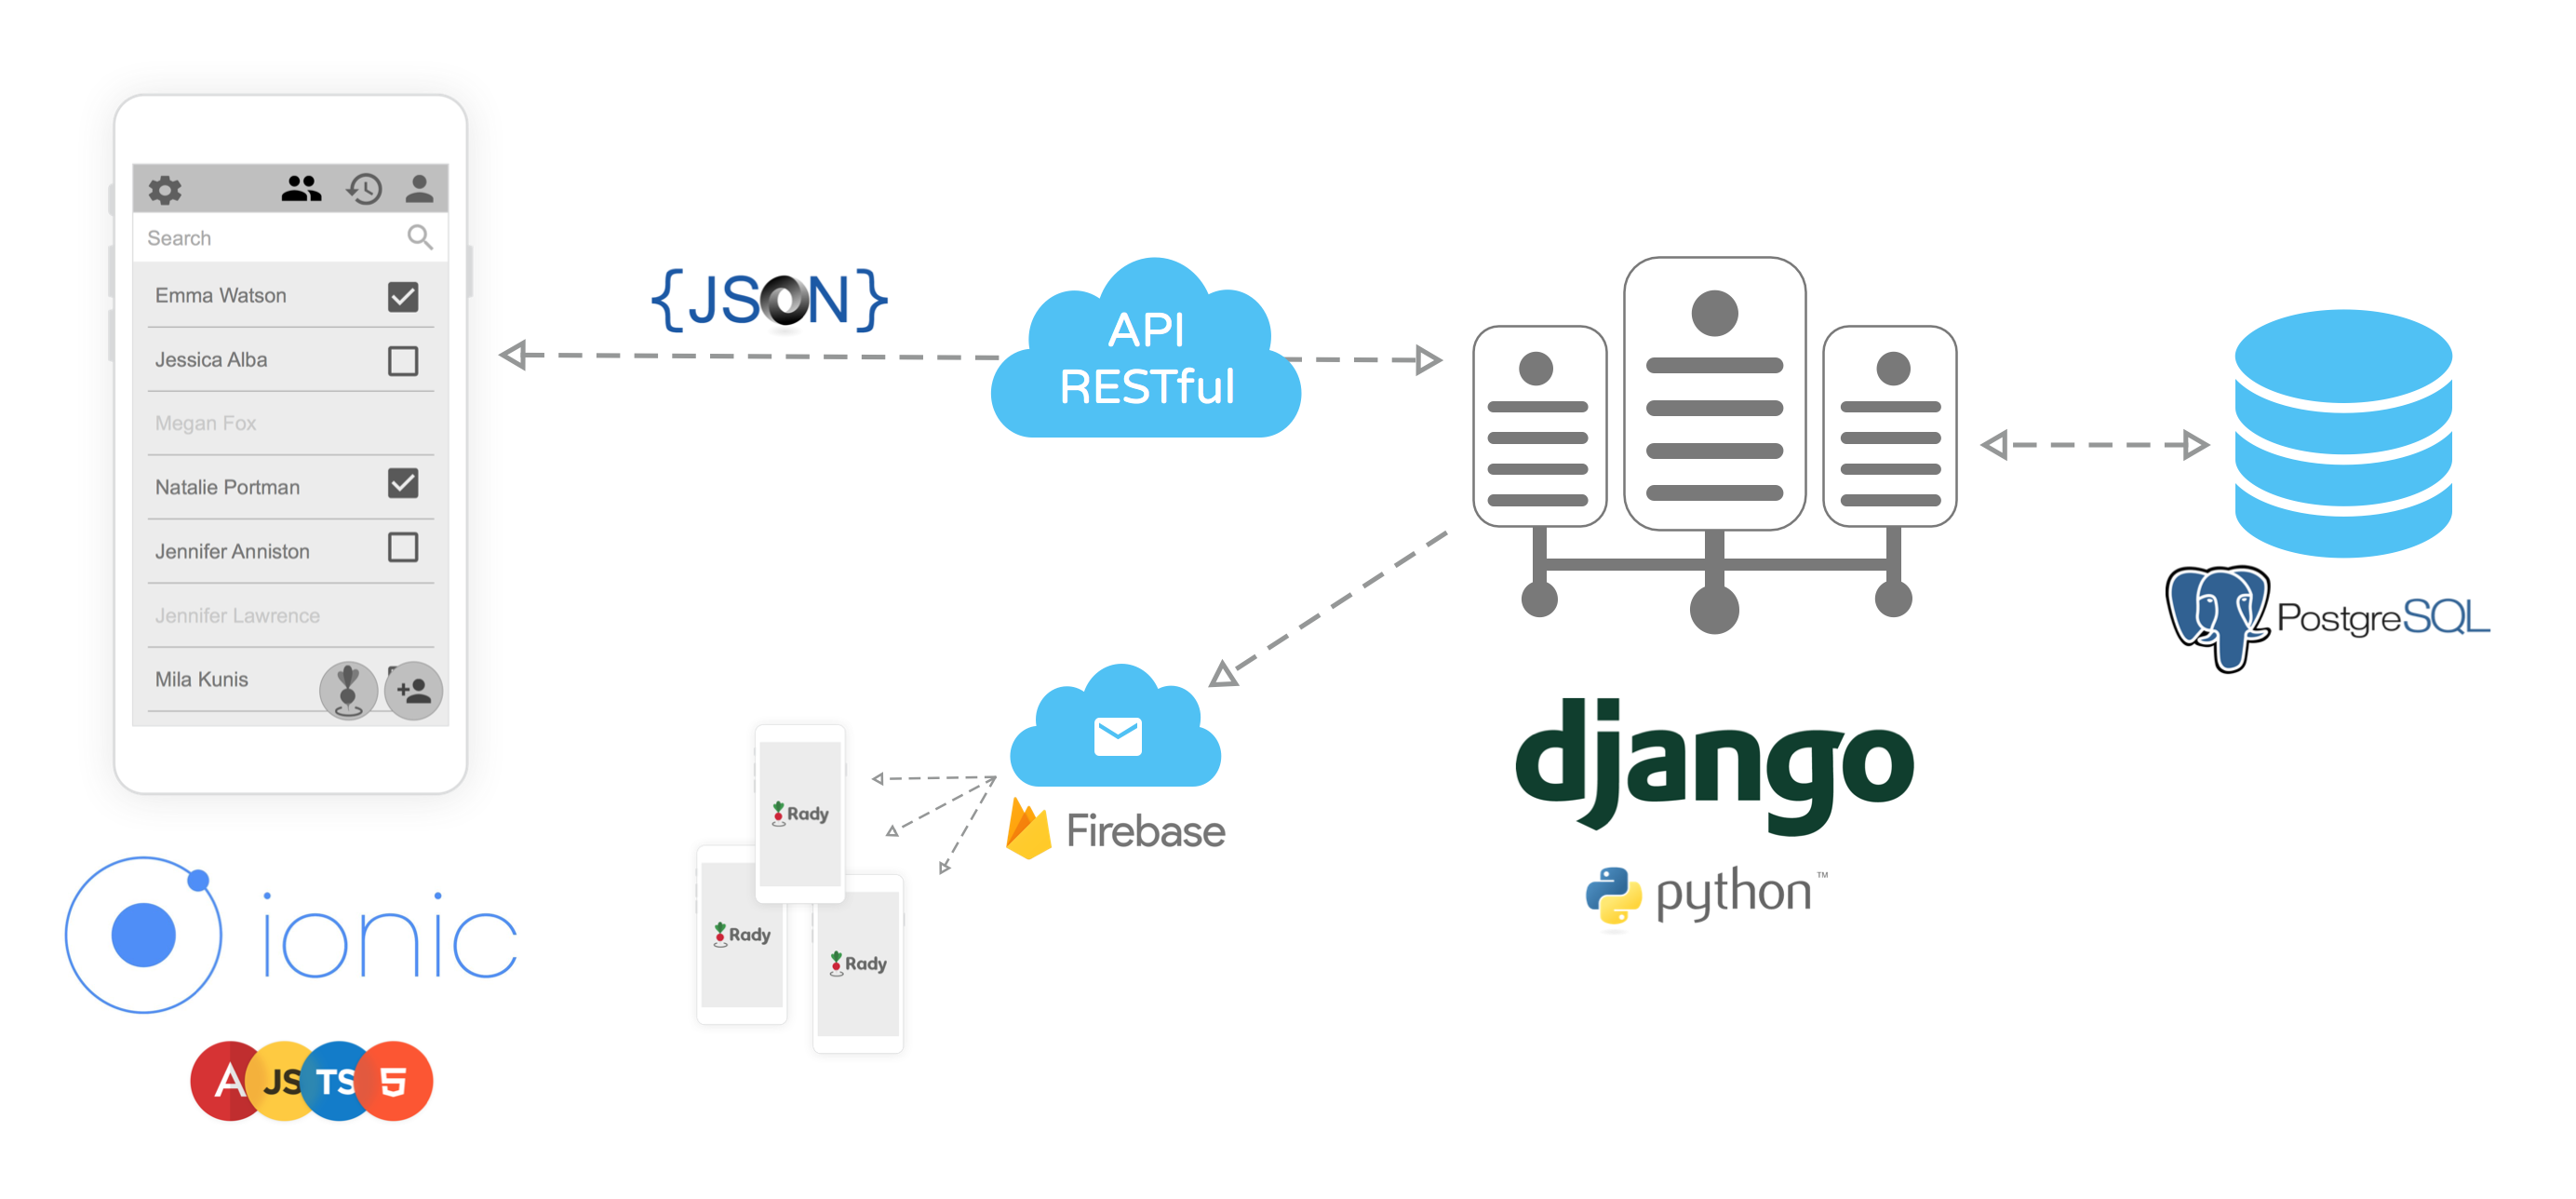
\includegraphics[scale=0.35]{../schema/schema-techno.png}
			\caption{Architecture et Technologies}
			\label{Architecture et Technologies}
		\end{figure}
		
	
	\section{Cadre de développement} 
		Le client de l'application a été développé en TypeScript(2.0.9) et angular(2.2.1), avec node.js(6.9.1) et le gestionnaire de paquet npm(3.10.9). Le serveur quand à lui a été développé avec python(3.5.2). 
		Nous avons également utilisé un service web d'hébergement et de gestion de développement de logiciels : GitHub avec le logiciel de gestion de version Git afin de gérer la mise en commun du code et l'intégration des différentes fonctionnalités au projet.
		Par ailleurs nous avons aussi utilisé un serveur d'integration continue (Travis) afin de pouvoir vérifier en temps réel le bon déroulement de notre projet
		Enfin nous avons mis en place des séries de tests visant à faire en sorte que l'api fournie par le serveur soit utilisable et ne contienne pas de faille.
			
	\section{Application Client}
	
	Lors du développement de notre application, la première étape a été de nous familiarier avec les différentes technologies et "frameworks" necessaire à la réalisation du produit final. Ensuite nous avons décidé de réaliser une maquette de l'interface que l'utilisateur final utilisera. Cette maquette a été conçu pour être simple et permettre une utilisation intuitive de l'application. Enfin il a fallut développer les menus et interfaces de l'application et lier les contrôleurs aux différentes fonctionalités
	
	\subsection{Frameworks}
	
	\subsubsection{Ionic2}
	
	\begin{figure}[H]
		\centering
		
\includegraphics[scale=0.45]{../images/ionic2-logo.png}
		\caption{Ionic2 logo}
		\label{Ionic2 logo}
	\end{figure} 
	
	Notre application a été réalisé avec le framework Ionic2. Ce framework, disponible depuis spetembre 2016, se distingue de sa version précédente Ionic en incluant la syntaxe ES6 , une nouvelle structure de fichier et en intégrant une CLI plus perfectionné permettant la génération automatique de pages.
	L’interface graphique est décrite par un fichier HTML utilisant des composants spécifique a Ionic2 :
	
	\lstset{language = HTML5}
	\begin{lstlisting}
	<ion-component>
	\end{lstlisting}
	
	Les balises permettent de placer les différents éléments de l’interface un peu à la manière dont on structure une page en HTML standard. La personnalisation des éléments se fait grâce à des styles CSS, spécifiés soit dans les attributs des éléments, soit via des feuilles de style externes dans les fichiers SCSS. Les attributs du SCSS diffèrent un peu des attributs CSS standards, ils permettent d'utiliser les SASS (Syntactically Awesome Style Sheets). Les fichier SCSS seront utilisé pour regénérer le CSS necessaire à l'affichage des styles. 
	A chaque fichier HTML et SCSS vient s’ajouter un fichier de code TypeScript, qui sert de contrôleur pour l’interface. Dans le HTML on définit les différents évènements de l’interface (par exemple un clic sur un bouton, ou un changement d'état d'un élément de type bascule) en déclenchant un appel de méthode au niveau du fichier contrôleur (le ficher TypeScript), qui gère ensuite l’évènement. Il est également possible d’ajouter et modifier des balises HTML directement depuis le contrôleur TypeScript afin de rendre l’interface plus dynamique, en la faisant par exemple réagir aux interactions de l’utilisateur ou aux réponses du serveur. 
	
	Voici la structure des sources de l'application mobile :
	
	\begin{figure}[H]
		\centering
		\dirtree{%
			.1 src/\DTcomment{répertoire contenant les sources de l'application}.
			.2 app/\DTcomment{répertoire contenant les liens des différents composant de l'application}.
			.3 app.component.ts\DTcomment{fichier définissant la page d'accueil de l'application}.
			.3 app.html\DTcomment{permet de lancer la page d'accueil de l'application}.
			.3 app.modules.ts\DTcomment{permet de charger les différents modules et interfaces de l'application}.
			.3 app.scss\DTcomment{styles portant sur toute l'application}.
			.3 main.ts\DTcomment{fichier permettant le lancement de l'application}.
			.2 assets/\DTcomment{répertoire contenant les éléments utiles à l'application}.
			.2 lib/\DTcomment{répertoire contenant les librairies utilisés par l'applcation}.
			.2 models/\DTcomment{répertoire contenant les modèles(classes) utilisés par l'application}.
			.2 pages/\DTcomment{répertoire contenant les différentes interfaces de l'application}.
			.3 add-contact/\DTcomment{répertoire contenant les éléments pour l'interface d'ajout de contact}.
			.4 add-contact.html/\DTcomment{code html définissant les composant de l'interface}.
			.4 add-contact.scss/\DTcomment{styles s'appliquant aux composant html}.
			.4 add-contact.ts/\DTcomment{logique appelé par les composants html}.
			.3 contact-list/\DTcomment{répertoire contenant les éléments pour l'interface de gestion de contact}.
			.4 contact-list.html/\DTcomment{code html définissant les composant de l'interface}.
			.4 contact-list.scss/\DTcomment{styles s'appliquant aux composant html}.
			.4 contact-list.ts/\DTcomment{logique appelé par les composants html}.
			.3 <...>\DTcomment{autres fichiers d'implémentation}.
			.2 providers/\DTcomment{répertoire contenant les services utilisés par l'applcation}.
			.2 theme/\DTcomment{répertoire contenant les fichiers .scss appliqués sur toute l'application}.
			.2 declarations.d.ts\DTcomment{fichier de déclaration pour le compilateur TypeScript}.
			.2 index.html\DTcomment{premiere page chargé par ionic permettant le chargement du reste de l'application}.
			.2 manifest.json\DTcomment{données pour l'affichage de l'application}.
			.2 service-workers.js\DTcomment{fichier contenant un script qui tournera en tache de fond}.	
		}
	\end{figure}
	
	On observe que les interfaces sont dans le dossier pages avec leurs ficher HTML, SCSS, et TS correspondant. Dans le dossier app/ on retrouve le lien entre les différentes pages et l'application en elle même. Ionic2 propose une hiérarchie intuitive regroupant les éléments par nature puis par fonctionnalité (librairies, models ...) afin de simplifier le développement.
	
	\subsubsection{Angular2}
	
	\begin{figure}[H]
		\centering
		
\includegraphics[scale=0.4]{../images/angular2-logo.png}
		\caption{Angular2 logo}
		\label{Angular2 logo}
	\end{figure} 
	
	AngularJs est un framework JavaScript conçu pour simplifier le developpement d'interfaces web. Ionic2 nous permet d'utiliser la version 2 de ce framework elle aussi sortie en septembre 2016. 
	Angular2 nous offre la possibilité de réaliser du "data binding" bidirectionnel. C'est a dire que lorsque les données affichés dans la vue sont modifé celà affecte directement le controlleur qui s'est mis à jour. Ce framework nous donne aussi accès à des directives rendant le code plus extensible et modulable, et nous permet d'utiliser l'injection de dépendance pour l'appel à des services initialisé ailleurs dans le code. 
	
	\subsubsection{Cordova}
	
	\begin{figure}[H]
		\centering
		
\includegraphics[scale=0.4]{../images/cordova-logo.png}
		\caption{Leaflet logo}
		\label{Leaflet logo}
	\end{figure} 
	
	Apache Cordova est un framework open-source qui permet de créer des applications pour différentes plateformes (Android, Firefox OS, iOS, Ubuntu, Windows 8...) en HTML, CSS et JavaScript. C'est lui qui sera appelé par Ionic pour "build" et déployer l'application directement sur le materiel.
	Ce framework permet d'avoir accès aux différentes fonctionnalités et élément du téléphone tel que la boussole, l'accéléromètre, la géolocalisation ou encore l'appareil photo.
	
	\subsubsection{Leaflet}
	
	Leaflet est une librairie open-source JavaScript pour le déeloppement d'application web de cartographie.
	
	\begin{figure}[H]
		\centering
		
\includegraphics[scale=0.4]{../images/leaflet-logo.png}
		\caption{Leaflet logo}
		\label{Leaflet logo}
	\end{figure} 
	
	
	Cette librairie nous permet non seulement d'afficher une carte mais aussi des marqueurs que nous utilisons pour afficher les positions des utilisateurs et lieux que nous souhaitons localiser. De plus celle-ci est extrêmement configurable, on peut en effet choisir d'utiliser nos propres éléments à afficher tel que des marqueurs personnalisé ou encore utiliser divers générateur de carte tel que mapbox, openstreetmap ou encore google map.
	
	\begin{figure}[H]
		\centering
		
\includegraphics[scale=0.4]{../images/mapbox-logo.png}
		\caption{Mapbox logo}
		\label{Mapbox logo}
	\end{figure} 
	
	\subsection{Design}
	
	Il a tout d'abord fallut établir le design de l'application comprenant les différentes interfaces à afficher, l'ordre d'affichage des ces interface ainsi que les animation et écrans de chargement à afficher. Ainsi nous avons commencé le projet par établir un flux d'utilisation
	
	\begin{figure}[H]
		\centering
		\includegraphics[scale=0.6]{../user-flow/user-flow-1.png}
		\caption{User flow - Loading}
		\label{User flow - Loading}
	\end{figure}
	
	\begin{figure}[H]
		\centering
		\includegraphics[scale=0.6]{../user-flow/user-flow-2.png}
		\caption{User flow - Sign in}
		\label{User flow - Sign in}
	\end{figure}
	
	\begin{figure}[H]
		\centering
		\includegraphics[scale=0.55]{../user-flow/user-flow-3.png}
		\caption{User flow - Main app}
		\label{User flow - Main app}
	\end{figure}
	
	\begin{figure}[H]
		\centering
		\includegraphics[scale=0.55]{../user-flow/user-flow-4.png}
		\caption{User flow - New Contact}
		\label{User flow - New Contact}
	\end{figure}
	
	\begin{figure}[H]
		\centering
		\includegraphics[scale=0.6]{../user-flow/user-flow-5.png}
		\caption{User flow - Gathering}
		\label{User flow - Gathering}
	\end{figure}
	
	
	\subsection{Developpement de l'interface}
	\subsubsection{Création des pages}
	
	Le développement des différentes pages a été réalisé en parallèle en répartissant les différentes écrans constituant les interfaces finales de notre application.
	La construction des interfaces des menus constituaient la partie la plus simple du développement car ils ne font appel que a des composants simple définit par Ionic2 et seulement quelques directives Angular2. 
	Nous nous sommes efforcé de réaliser des pages les plus proches possible du design réalisé précédemment afin de garder une simplicité de l'interface tant au niveau du développement que au niveau de l'utilisation finale. 
	
	\begin{figure}[H]
		\centering
		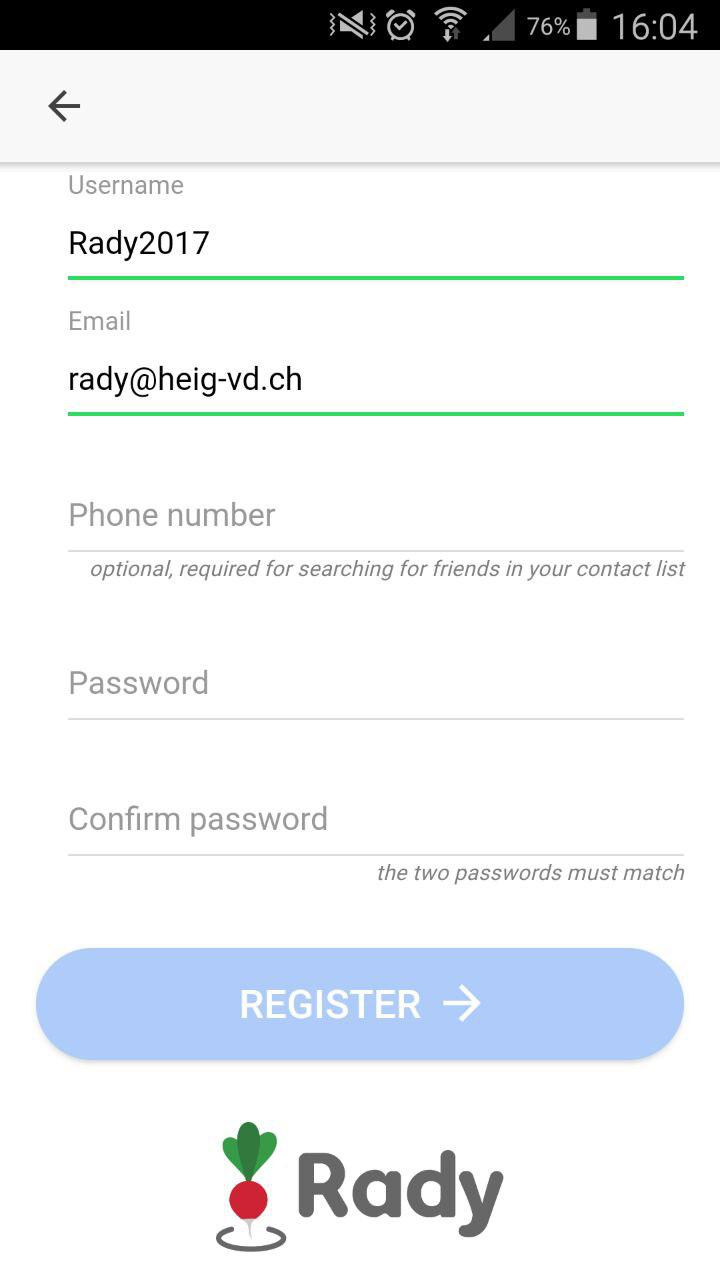
\includegraphics[scale=0.20]{../screenshot/screenshot-register.jpg}
		\caption{Capture d'écran - Enregistrement}
		\label{Capture d'écran - Enregistrement}
	\end{figure} 	 
	
	\newpage
	
	Ensuite est venu l'implémentation des différentes fonctions appelé par les éléments graphiques (vérification des champs, communication avec le serveur, changement de page). Pour ce faire nous avons du créer et utiliser différentes librairies et validateurs.
	
	\subsubsection{Validateurs}
	
	Modularité
	Il n'existaient pas 
	Phone - Email - Match
	
	Pour éviter d'effectuer des appels serveur inutile nous avons choisi de faire des tests sur la forme des saisies utilisateur directement dans l'application avant de les envoyer au serveur via l'API afin de diminuer le nombre de réponses négatives. Pour effectuer ces tests nous avons donc eu besoin d'une librairie de validateurs pour nous permettre de définir si la saisie possède la bonne forme ou non. 
	Étant donné que nous n'avons pas trouvé de validateurs correspondant à nos attentes nous avons décidé de les implémenter à la main.
	
	\begin{lstlisting}[style=htmlcssjs]
	/**
	* Email validator
	* Check if the control is a valid email
	* @param emailcontrol
	* @param msg
	*/
	public static email(emailcontrol: string, msg: string) {
		return (group: FormGroup): ValidatorResult => {
			if(group.get(emailcontrol).value.length === 0)
				return null;
			let errors = {};
			let regExp = /[a-z0-9!#$%&'*+/=?^_`{|}~-]+(?:\.[a-z0-9!#$%&'*+/=?^_`{|}~-]+)*@(?:[a-z0-9](?:[a-z0-9-]*[a-z0-9])?\.)+[a-z0-9](?:[a-z0-9-]*[a-z0-9])?/;
			if(!regExp.test(group.get(emailcontrol).value))
			errors[emailcontrol] = msg;
			return Object.keys(errors).length === 0 ? null : errors;
		}
	}
	\end{lstlisting}
	
	Dans ce validateur pour les e-mail nous utilisons une expression régulière afin de déterminer si l'e-mail entré par l'utilisateur possède une forme correcte. Lorsque le validateur détecte que l'email n'est pas valide il renvoie une erreur à l'utilisateur qui est instantanément averti.
	
	Nous utilisons aussi un validateur personalisé pour les numéro de téléphone afin de déterminer si le numéro est valide suivant l'indicatif du pays. 
	\begin{lstlisting}[style=htmlcssjs]
	/**
	* Phone validator
	* Check if the control the a valid phone
	* @param phonecontrol
	* @param countrycontrol
	* @param msg
	*/
	public static phone(phonecontrol: string, countrycontrol: string, msg: string) {
		return (group: FormGroup): ValidatorResult => {
			if(group.get(phonecontrol).value.length === 0)
				return null;
			let errors = {};
			try {
				const phoneUtil = libphonenumber.PhoneNumberUtil.getInstance();
				const phoneNumber = phoneUtil.parse(group.get(phonecontrol).value, group.get(countrycontrol).value);
				if(!phoneUtil.isValidNumber(phoneNumber))
					errors[phonecontrol] = msg;
				} catch(e) {
					errors[phonecontrol] = msg;
			}
			return Object.keys(errors).length === 0 ? null : errors;
		}
	}
	\end{lstlisting}
	
	Cette fois-ci nous n'utilisons pas d'expression régulière mais nous faisons appel à une librairie externe : libphonenumber.
	Cette librairie permet de passer le numéro de téléphone sous forme canonique avant de vérifier la cohérence de celui-ci ce qui nous permet de garantir une uniformité de la nature des numéros de téléphne d'un utilisateur à un autre.
	
	 
	
	\subsubsection{Rencontres}
	
	TODO : EXPLICATION + CODE
	
	\subsubsection{Calculs des parcours}
	
	TODO : EXPLICATION DE ALGO
	
	
	\section{Serveur et Communication}	
	\subsection{Fonctionnement General}
	
	TODO : EXPLIQUER COMMENT ON COMMUNIQUE -> API -> PUSH
	TODO : SCHEMA DE COMMUNICATION ENTRE LES APPAREIL 
	
	\subsection{Base de donnée}
	\subsubsection{Tables}
	
	TODO : SCHEMA DES TABLES
	TODO : Explication de la création des tables 
	
	\subsubsection{Connection avec Django}
	
	TODO : EXPLICATION DU FONCTIONNEMENT DE DJANGO AVEC POSTGRESQL
	
	\subsection{Api}
	
	TODO : LISTING DES DIFFERENTES API A DISPOSITION
	
	\subsection{Notifications}
	\subsubsection{Fonctionement}
	
	TODO : EXPLICATION DU SYSTEME DE PUSH
	
	\subsubsection{Firebase Cloud Messaging}
	
	TODO : EXPLICATION DE L'INTEGRATION DE FCM + CODE
	
	
	
	\section{Sécurité}
	
	TODO : EXPLIQUER EN QUOI C'EST IMPORTANT
	
	\subsection{Communication}
	
	TODO : CHIFFREMENT + CODE
	
	\subsection{Tests Unitaires}
	\subsubsection{Tests API}
	
	TODO : FONCTIONNEMENT DES TESTS + CODE
	
	\subsubsection{Tests du Push}
	
	TODO : FONCTIONNEMENT DES TESTS + CODE
	
	\subsubsection{Coverage}
	
	TODO : EXPLICATION DU COVERAGE + SCREENSHOT 97\%+ COVERAGE
	
		\section{Conclusion}
		% Conclusion critique sur l'application fournie et le travail de groupe
		% Indications précises de ce qui ne fonctionne pas correctement
		% Propositions d'améliorations pour des développements futurs
		
		\subsection{Application fournie}			
		Vis à vis du cahier des charges initial (disponible en annexe), l'application répond à toutes les fonctionnalités prévues hormis l'implémentation de certains algorithmes, dont voici la liste:
		\begin{itemize}
			\item Arborescence recouvrante de poids min
			\item Arborescence recouvrante de section min/max
			\item Flot de capacité fixée (ou min)
			\item Flot de capacité fixée (ou min) de poids min
		\end{itemize}
		Les fonctionnalités optionnelles et futures n'ont pas pu être intégrées par manque de temps, cependant leur ajout est tout à fait réalisable car la conception générale de l'application a été prévue pour être ouverte aux extensions. Notons encore que l'interface graphique n'est pas tout à fait la même que la maquette présente dans le cahier des charges, néanmoins les fonctionnalités sont les mêmes.\\
		
		Concernant la stabilité du programme, la majorité des bugs/crashs découverts pendant le projet a été corrigée. Cependant certains cas posent toujours problème:
		\begin{enumerate}
			\item Un graphe ne possédant pas tous les sommets dans l'ordre (ex: \texttt{g=dfs(\{\#2\}, 1);}) pose problème à certaines fonctionnalités (ex: \texttt{draw(g);}, \texttt{egli::deserialize(...);})
			\item Fuites mémoires détectées au niveau de la couche \textit{graphes et algorithmes}
			\item La fenêtre d'aide ne se ferme pas lorsque que l'on quitte la fenêtre principale (avec la croix en haut à droite)
			\item La grammaire du langage ne permet pas de tout faire (ex: \texttt{v=(0); g=\{v\};}, \texttt{v=(0::-1);}, \texttt{draw(dfs(g, 0)[0]);})
		\end{enumerate}
		Les cas (1) et (2) sont des priorités absolues pour la suite du développement, mais nous les avons malheureusement découverts trop tard pour pouvoir les corriger en l'état. Par chance, les causes des problèmes sont connues, ce qui permettra de les corriger rapidement. De plus, nous avons découvert l'existence du logiciel DrMemory \cite{drmemory} qui nous offre la possibilité de cibler les fuites mémoires très précisément.\\
		
		Un petit mot sur le langage développé spécifiquement pour l'application. Celui-ci demande un petit temps d'apprentissage, mais la prise en main est assez rapide. L'aide intégrée et ses pages bien expliquées (facilement extensible), sa fonction de recherche par mots-clés, ainsi que l'auto-complétion des fonctions et variables prend l'utilisateur par la main et rend l'utilisation de l'application agréable.\\  
		
		Au final, nous sommes satisfaits du résultat final bien qu'il reste encore d'importants bugs à corriger. Le projet offre de nombreuses possibilités d'amélioration, tant au niveau de l'interface graphique que du reste, et nous sommes très contents de cela. Voici une liste non-exhaustive des améliorations possibles auxquelles nous avons pensé:
		\begin{itemize}
			\item Meilleure visualisation des graphes
			\item Affichage des variables créées dans une zone de l'interface graphique
			\item Coloration syntaxique
			\item Fonctionnalités optionnelles et futures du cahier des charges
			\item ... et plein d'autres
		\end{itemize}
		
		\subsection{Planification}
		% Les figures ne prennent pas en compte les tests et la doc, uniquement la conception et l'impl.
		
		La planification initiale du projet (disponible en annexe) a fait ressortir plusieurs problèmes. Premièrement, les temps d'analyse et de conception ont été très largement sous-estimés, ce qui a engendré un gros décalage des tâches:
		\begin{figure}[H]
			\includegraphics[width=\textwidth]{Planification/comparaisondates.pdf}
			\caption{Comparaison entre les dates prévues et effectives des tâches principales}
			\label{fig:comparaisondates}
		\end{figure}
		On peut expliquer cela par deux choses: certains problèmes étaient plus complexes que prévus, et l'apprentissage de Qt était beaucoup plus long. En effet, Qt est très puissant et offre de multiples manières d'aborder un problème, en contre-partie cela induit des pertes de temps lorsque l'on part dans la mauvaise direction. Cependant une fois que Qt est pris en main, les gains lors de l'implémentation sont conséquents.\\ 
		
		Deuxièmement, la planification initiale était une suite de tâches à faire complètement avant de passer à la suivante. Dans les faits, les tâches (pour une même personne) ont été réalisées en parallèle, cela a impliqué une dissonance entre les temps prévus et les temps effectifs.\\
		
		Troisièmement, la partie sur les graphes et les algorithmes a été la plus largement sous-estimée, le graphique suivant le montre assez clairement:
		\begin{figure}[H]
			\includegraphics[width=\textwidth]{Planification/comparaisonheures.pdf}
			\caption{Comparaison entre le temps prévu et temps effectif des tâches
				principales}
			\label{fig:comparaisonheures}
		\end{figure}
		
		Pour finir, les différentes tâches, bien que mal planifiées, ont été bien cernées dès le début du projet. Cela a permis une séparation du travail correcte et indépendante, ainsi qu'une application finale utilisable. Nous sommes cependant convaincus qu'utiliser un modèle de développement itératif (et non pas en cascade) aurait apporté un plus au projet. En effet, cela nous aurait obligé à mettre les différentes couches en commun plus souvent, et ainsi détecter les problèmes avant la fin du projet. 
		
		\subsection{Travail de groupe}
		Le principal problème, comme mentionné dans la section précédente, a été le fait que nous n'avons pas fixé suffisamment de délais intermédiaires et que la mise en commun n'a été faite qu'à la fin du projet. Cela a posé des problèmes que nous n'avons malheureusement pas pu résoudre dans les temps.\\
		
		Le second problème a été un laxisme en début de semestre, nous avons donc dû fournir un gros effort lors des dernières semaines. Lors de ces "rushs", où nous avons travaillé tous ensemble dans la même pièce, il a été intéressant de constater la grande efficacité avec laquelle nous avons travaillé. En effet les problèmes se résolvent beaucoup plus vite et l'ambiance offre un cadre de travail beaucoup plus motivant et encourageant. Il nous semble donc important à l'avenir de planifier ce type de séance plus souvent tout au long d'un projet, pour une meilleure productivité.\\
		
		Pour conclure, ce projet a été une expérience enrichissante, autant du point de vue technique et de la planification, que du travail en grand groupe. La collaboration au sein de l'équipe a été très bonne durant toute la durée du semestre, et cela même malgré la grande charge de travail avec les autres cours. Nous sommes donc au final heureux d'avoir pu participer à l'élaboration de A à Z d'un projet complet et complexe, nous profitons de cette conclusion pour nous remercier les uns les autres pour le travail accompli.
		
		\newpage
	
	\newpage
	

			
	
	% Tables des figures
	\listoffigures
			
	% References
	\begin{thebibliography}{9}
		\bibitem{meteor}
		Open source platform for web, mobile, and desktop developpement. ,\\ \url{https://www.meteor.com/}
		
		\bibitem{ionic} 
		Web app developpement framework for mobile ,\\ \url{http://ionic.io/}
		
		\bibitem{django}
		High-level Python Web framework, \\ \url{https://www.djangoproject.com/}
		
		\bibitem{plantuml}
		PlantUML, Open-source tool that uses simple textual descriptions to draw UML diagrams,\\ \url{http://plantuml.com/}\\ \url{http://www.planttext.com/planttext}
		
		\bibitem{Graph data wikipedia.org}
		Graphs data structures,\\ \url{https://en.wikipedia.org/wiki/Adjacency_matrix#Data_structures}
		
		\bibitem{boost.spirit}
		Boost.Spirit (v2.5.2), is an object-oriented, recursive-descent parser and output generation library for C++,\\ \url{http://www.boost.org/doc/libs/1_60_0/libs/spirit/doc/html/index.html}
		
		\bibitem{tries}
		Robert Sedgewick, Kevin Wayne.\\
		\emph{Algorithms, fourth edition}\\
		\url{http://algs4.cs.princeton.edu/lectures/52Tries.pdf}
		
		\bibitem{sedgewick}
		Robert Sedgewick.\\
		\emph{Course on ternary search tries}
		\url{https://www.youtube.com/watch?v=CIGyewO7868}
		
		\bibitem{drmemory}
		DrMemory,\\
		\url{http://drmemory.org/}
	\end{thebibliography}
			
	\newpage
		
		
	\section{Annexes projet}
		\subsection{Cahier des charges}
			\includepdf[pages=-,width=\textwidth]{cahierdescharges}
		\subsection{Journaux de travail}
			\includepdf[pages=-,width=\textwidth]{journaldetravail}
		\subsection{Planification initiale}
			\includepdf[pages=1,angle=90,width=\textwidth]{Planification/gantt}	
			\includepdf[pages=2,angle=90,width=\textwidth]{Planification/gantt}	
			\includepdf[pages=3,angle=90,width=\textwidth]{Planification/gantt}	
			\includepdf[pages=4,angle=90,width=\textwidth]{Planification/gantt}	
			\includepdf[pages=5,angle=90,width=\textwidth]{Planification/gantt}	
			\includepdf[pages=6,width=\textwidth]{Planification/gantt}	

\end{document}
